\documentclass[utf8]{ctexart}
\usepackage{geometry}
\usepackage{graphicx}
\usepackage{amsmath} %数学公式
\usepackage{amssymb}             %数学公式             %数学字体
\usepackage{mathrsfs} 
\usepackage{txfonts}
\usepackage{float}  %设置图片浮动位置的宏包
\usepackage{subfigure}%插入多图时用子图显示的宏包
\geometry{a4paper,scale=0.80}
\author{左熙辰-2000012103}
\date{}
\title{植物学实验2}
\ctexset{
    section/name= {实验操作}
}
\begin{document}
    \maketitle
    \section{地钱植物的形态,结构和生殖}
    \subsection*{结果}
        \begin{figure}[h]
            \centering
            \subfigure[地钱颈卵器结构]{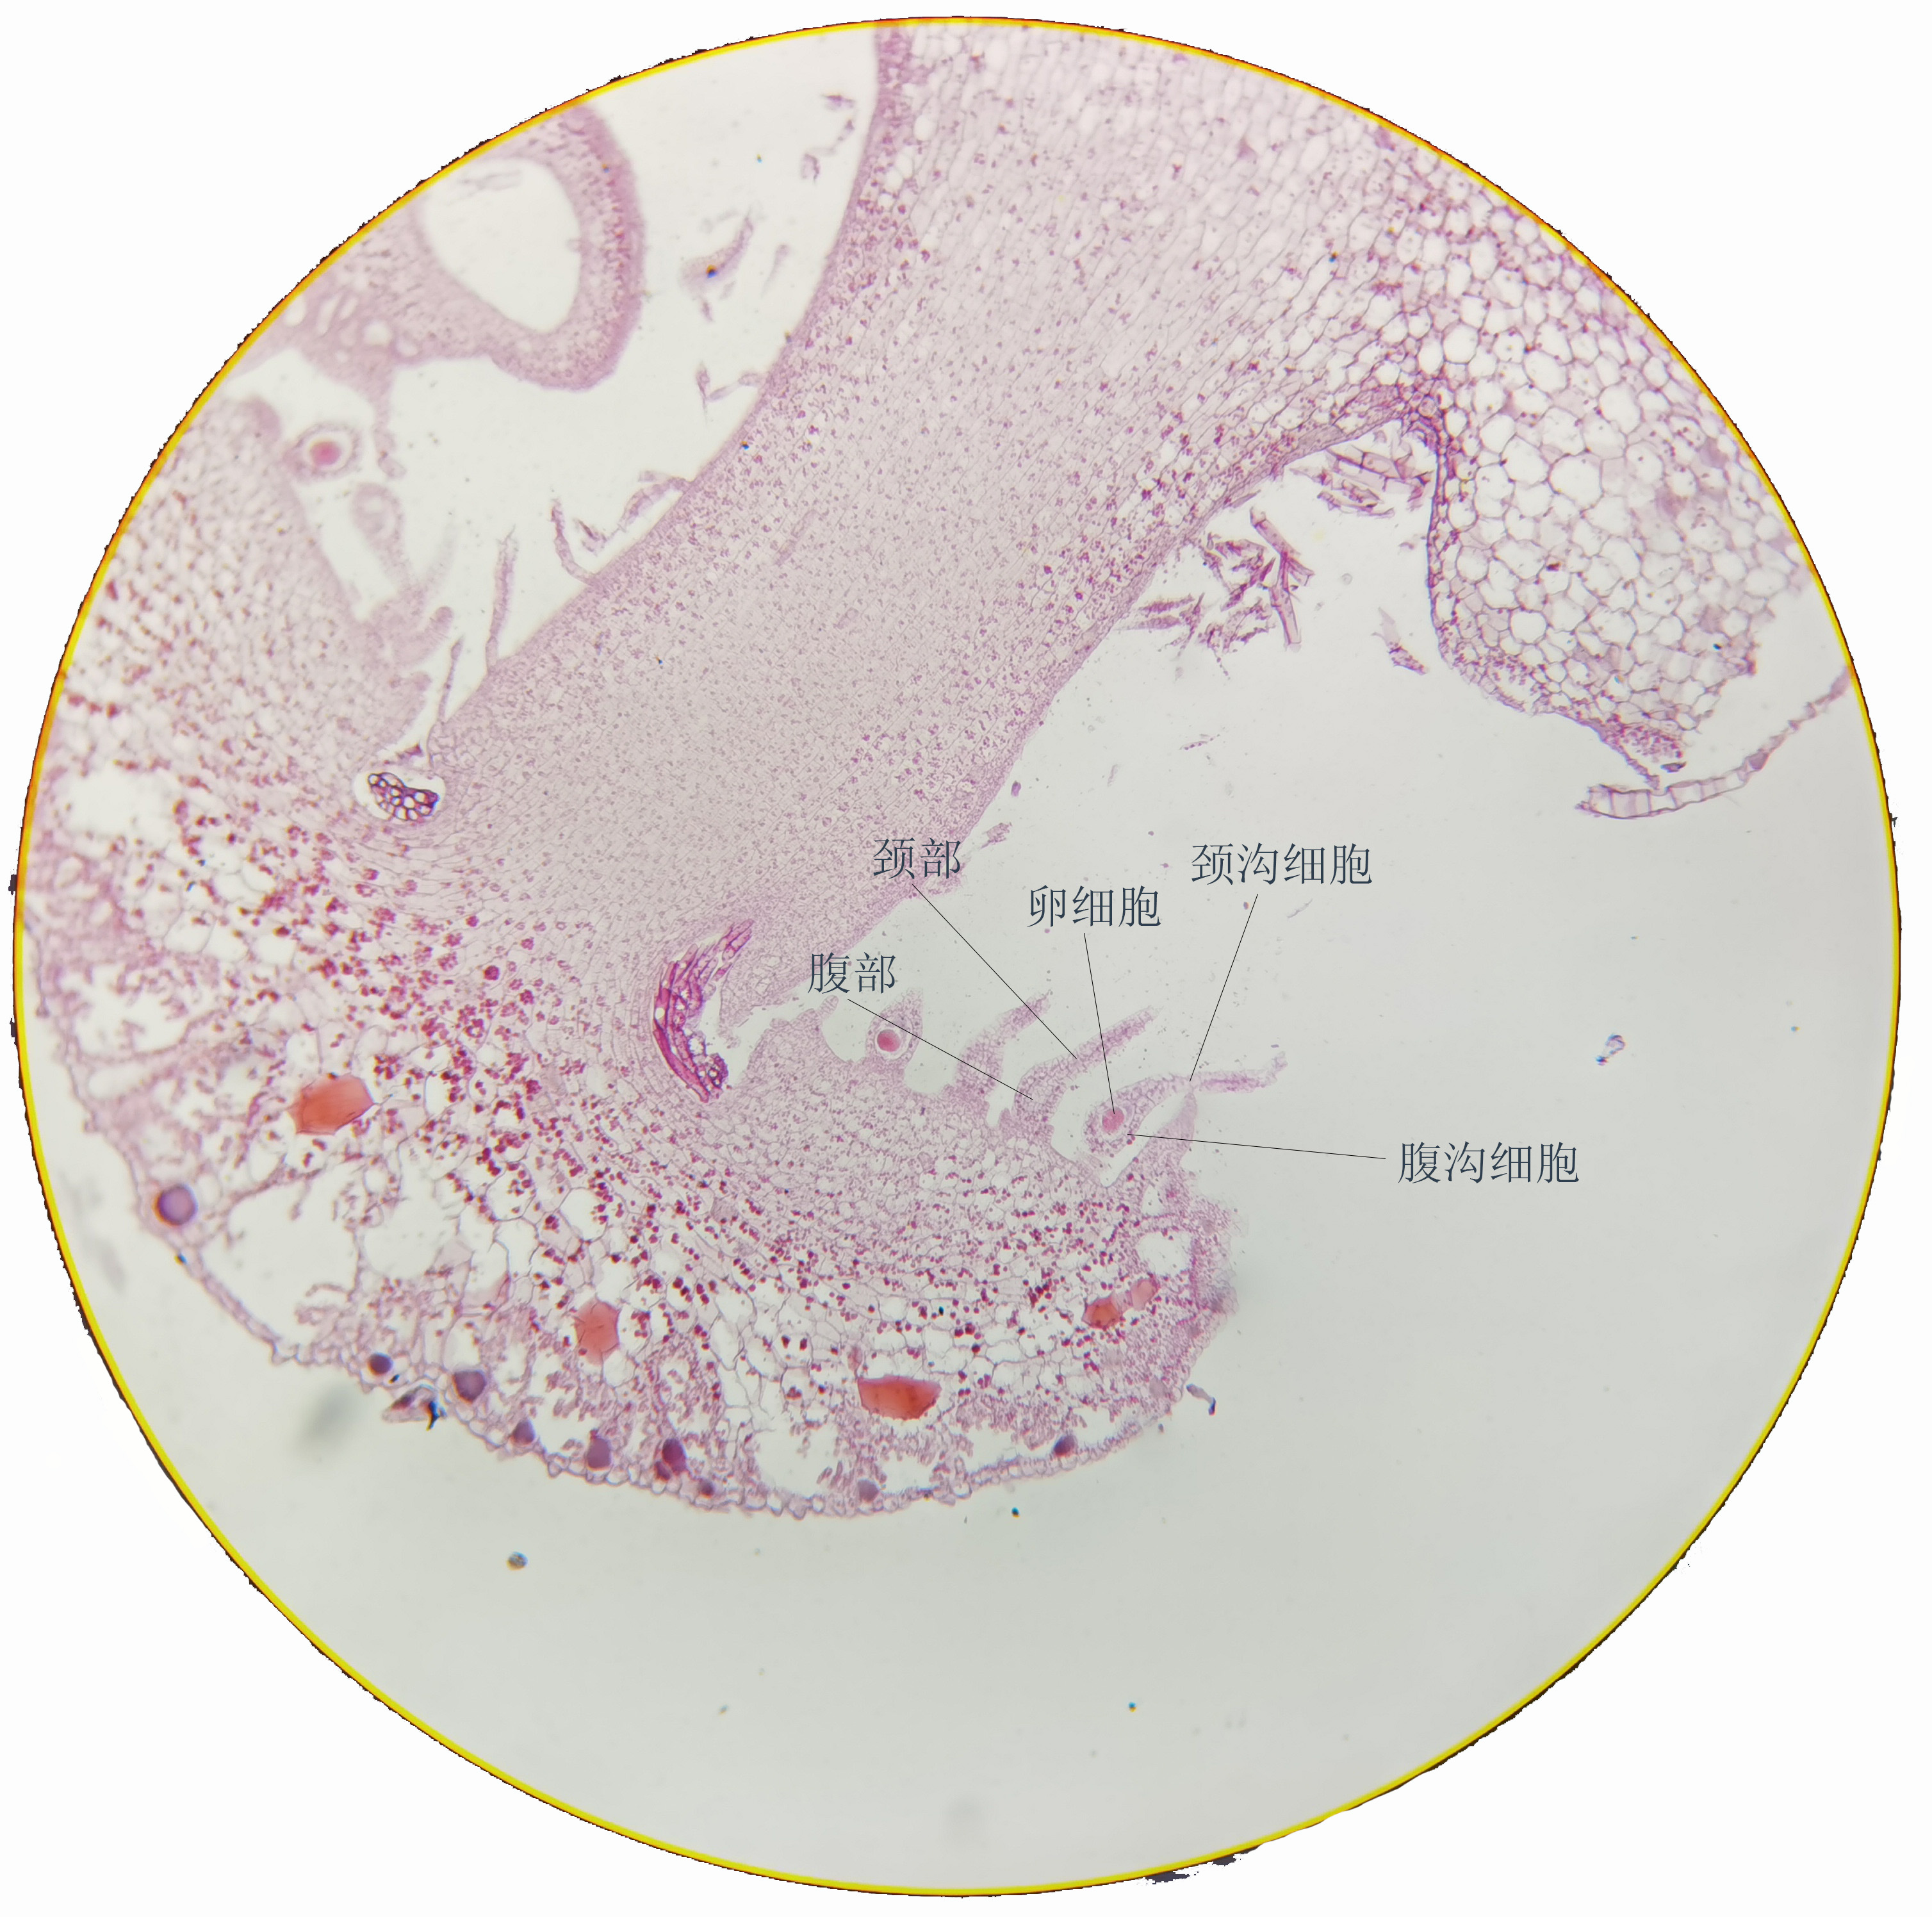
\includegraphics[scale=0.05]{src/botany/IMG_20201125_190734.jpg}
            \label{diqianpeizi}
            }
            \subfigure[地钱孢子体结构]{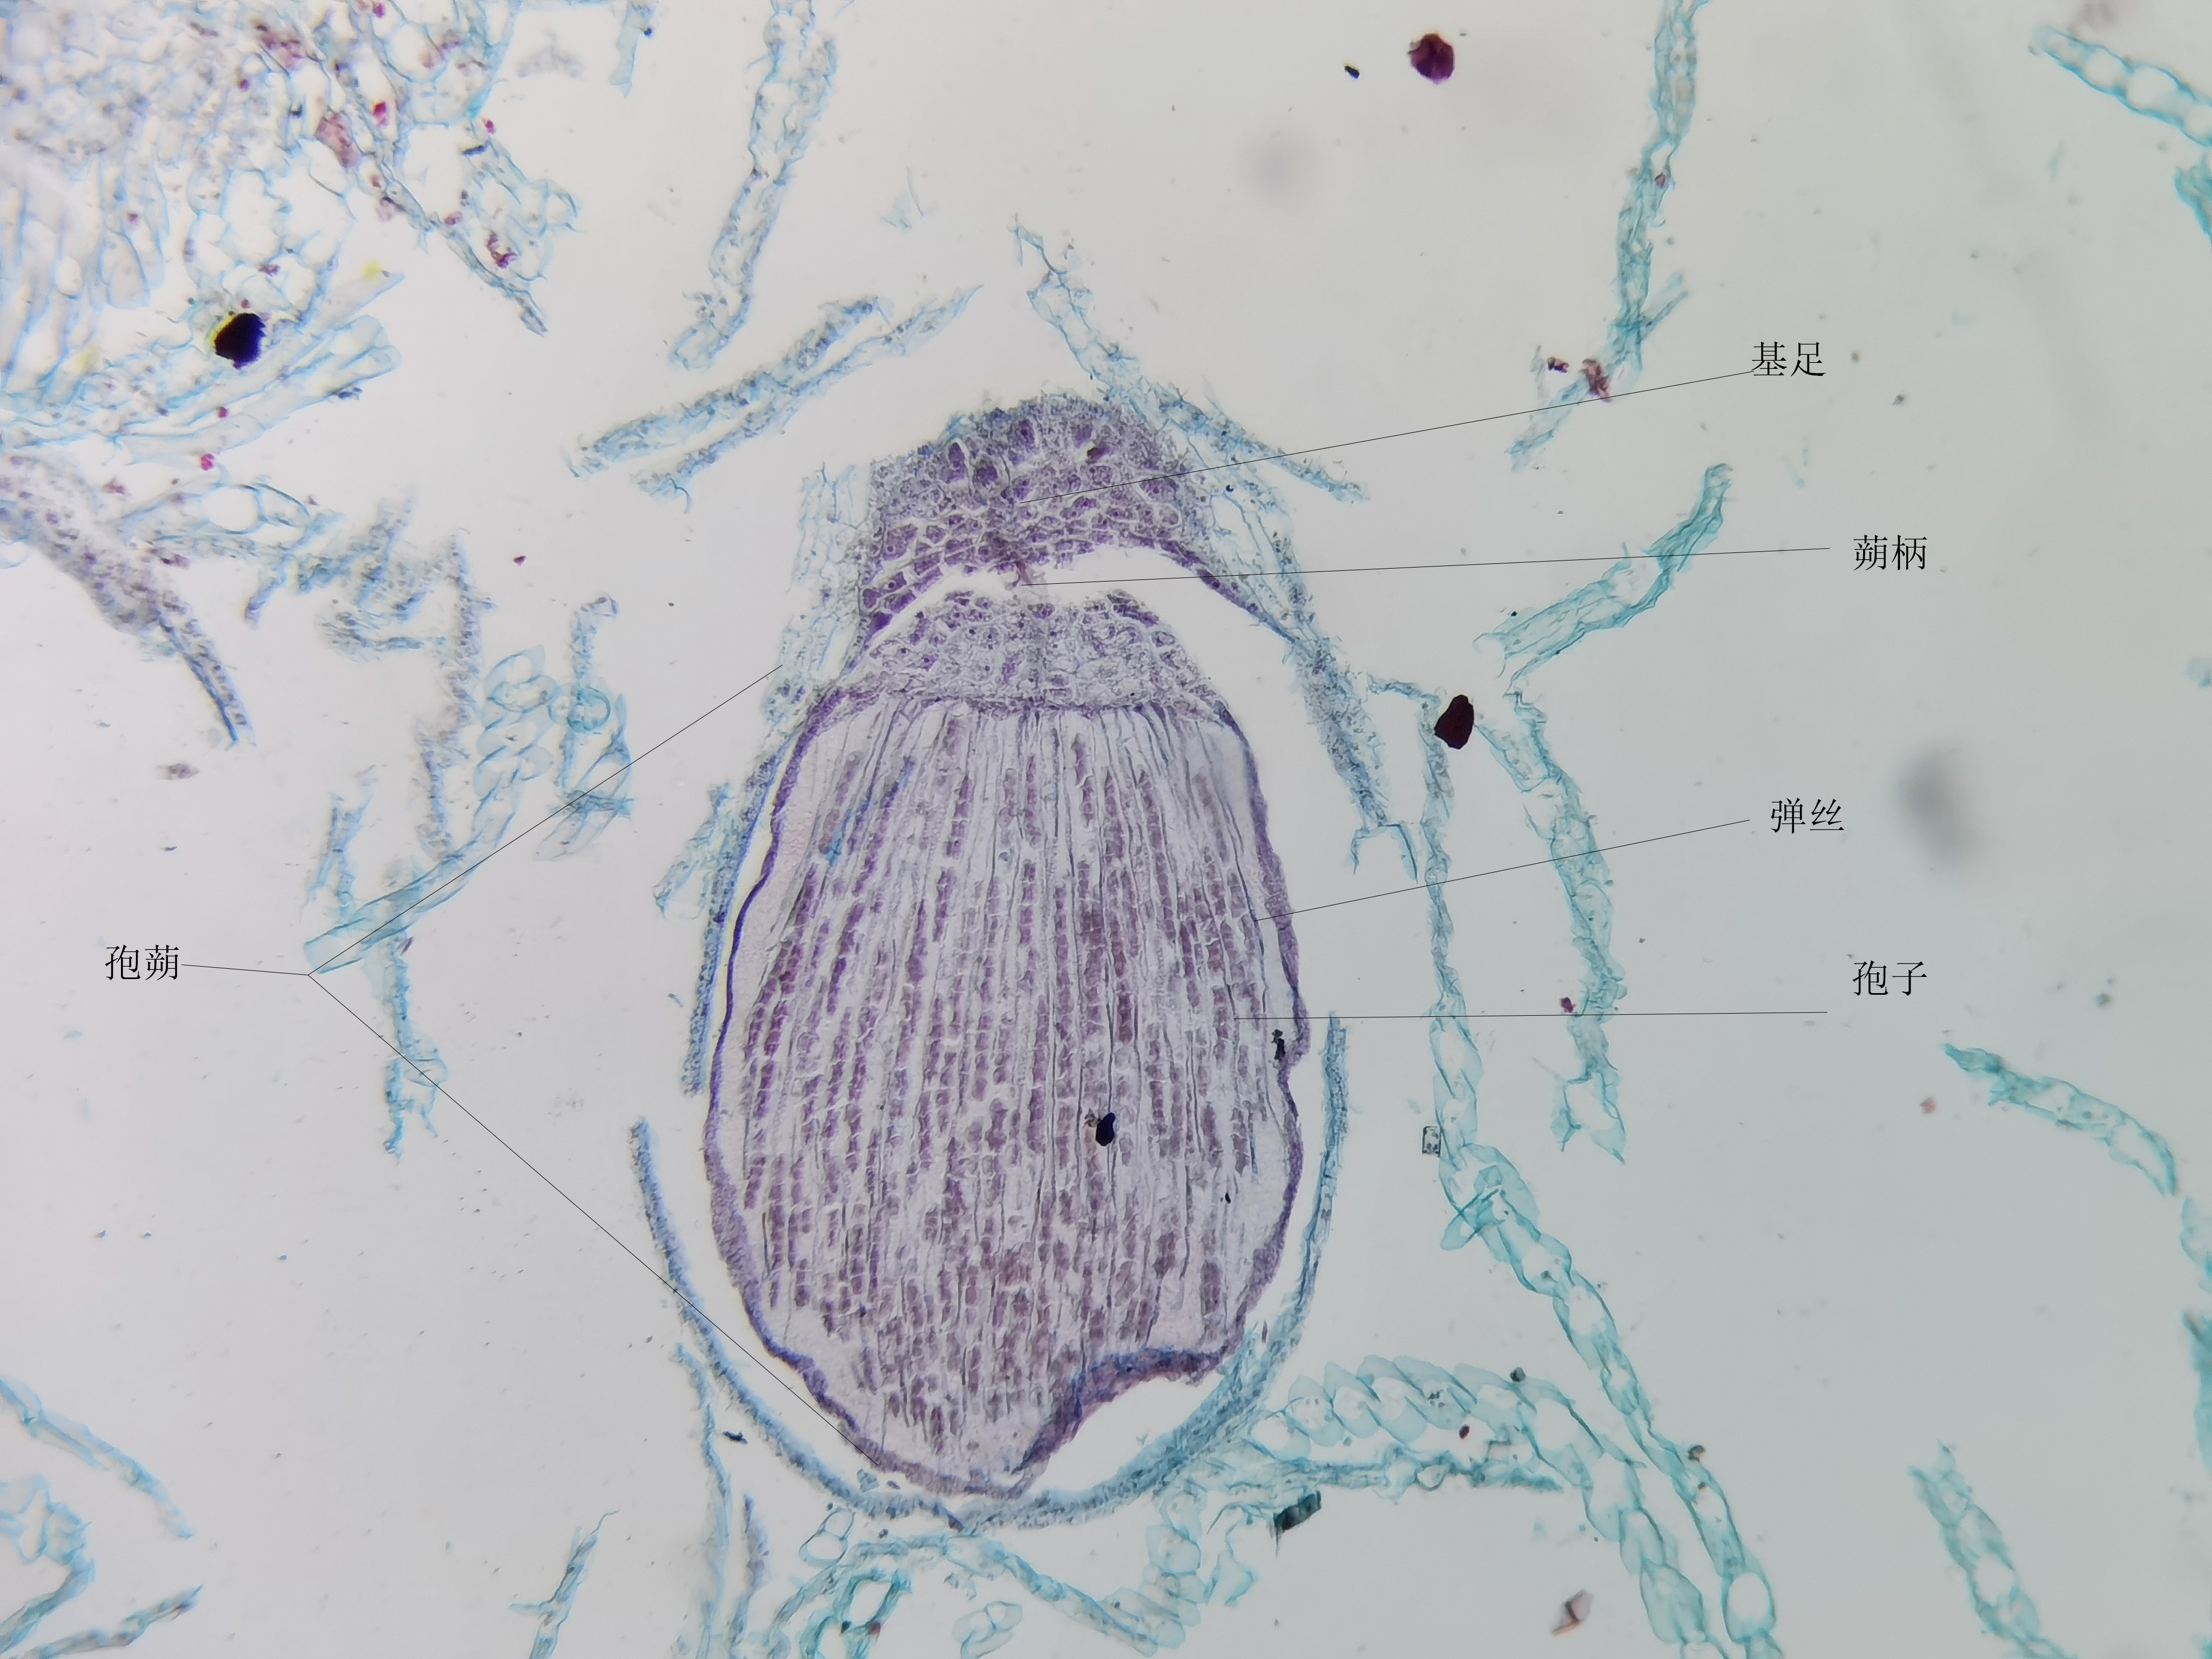
\includegraphics[scale=0.05]{src/botany/IMG_20201125_190311.jpg}\label{diqianbaoziti}}
            \caption{地钱生殖结构}
        \end{figure}
        \paragraph*{1.用简图或照片显示地钱颈卵器结构,包括颈部、腹部、预沟细胞、腹沟细胞和卵细胞等;}
        \paragraph*{答:}见\ref{diqianpeizi}
        \paragraph*{2.用简图或照片显示地钱孢子体各部分结构,包括孢蒴、蒴柄、基足、弹丝、孢子等.}
        \paragraph*{答:}见\ref{diqianbaoziti}
    \subsection*{讨论}
        \paragraph*{1.为什么地钱是高等植物?}
        \paragraph*{答:}因为其产生了胚
    \section{铁线蕨的形态,结构和生殖}
    \subsection*{结果}
    \begin{figure}[h]
        \centering
        \subfigure[铁线蕨孢子囊]{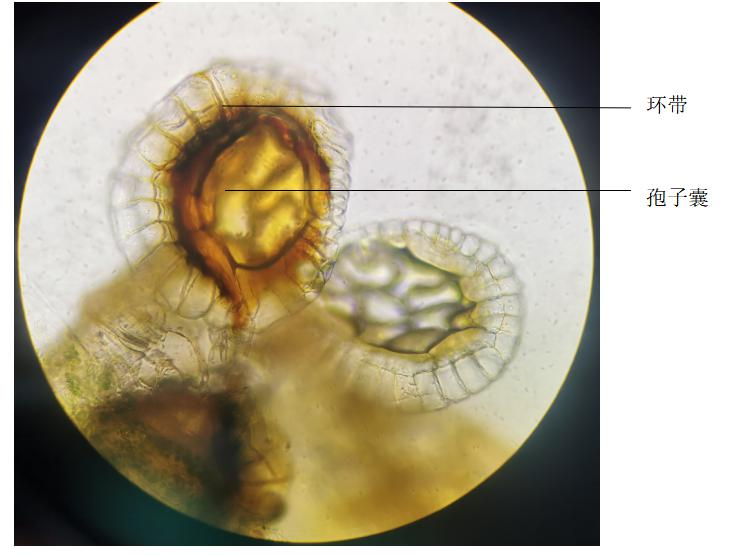
\includegraphics[scale=0.5]{src/botany/苔藓蕨类裸子植物实验报告juenang.jpg}\label{juebaonang}}
        \subfigure[铁线蕨孢子]{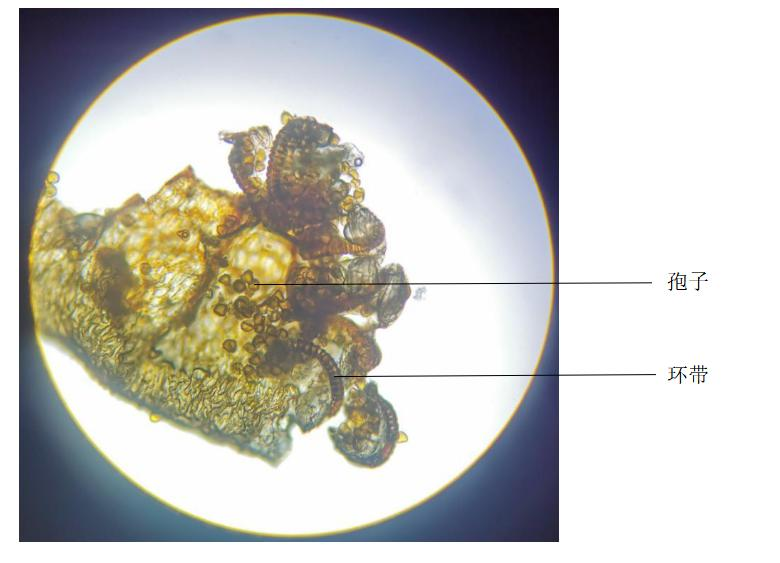
\includegraphics[scale=0.5]{src/botany/苔藓蕨类裸子植物实验报告王一博2000012255huand.jpg}\label{juebao}}
        \subfigure[铁线蕨配子体]{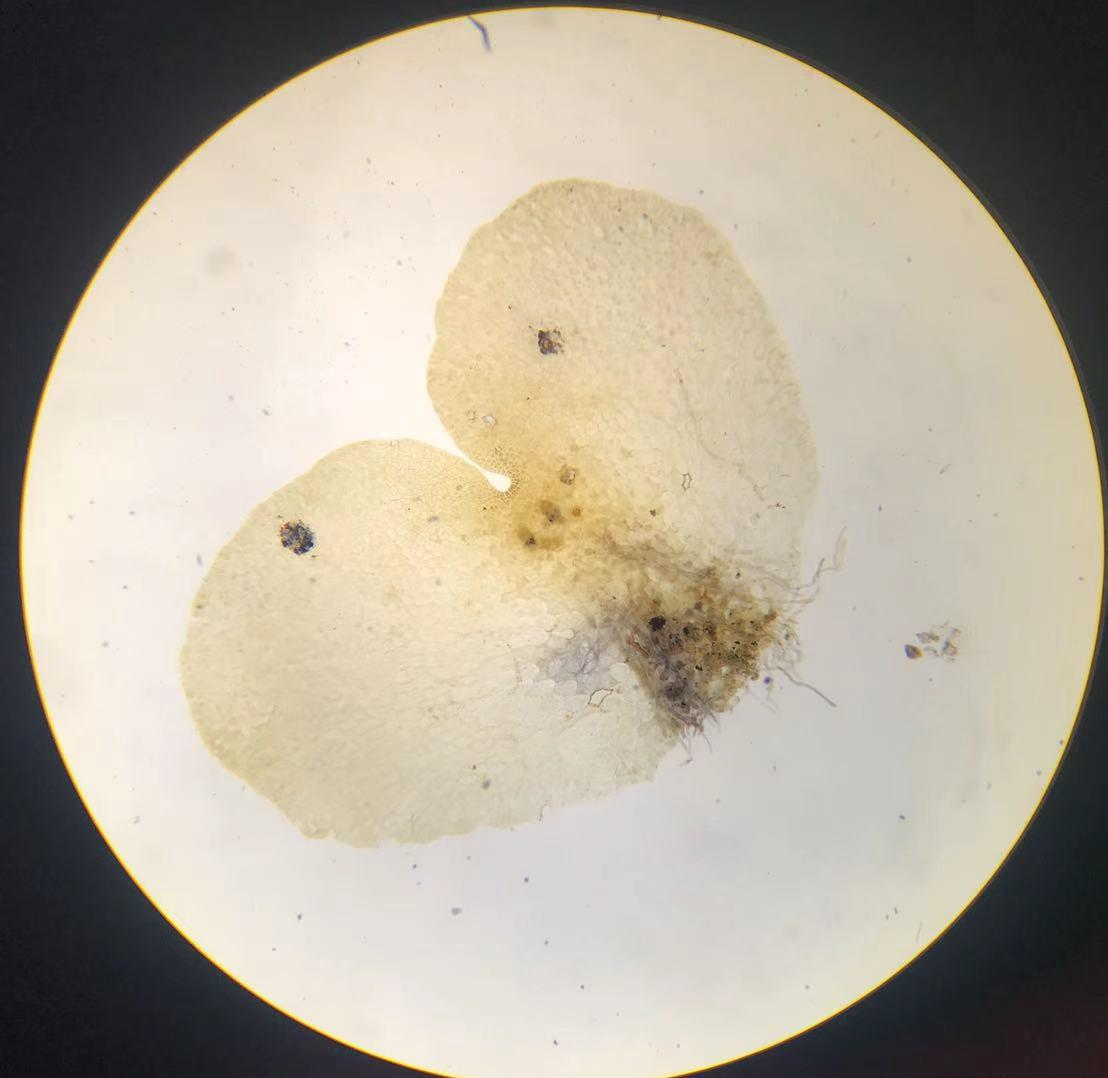
\includegraphics[scale=0.5]{src/botany/苔藓蕨类裸子植物实验报告王一博2000012255.jpg}\label{juepei}}
        \caption{铁线蕨生殖结构}
    \end{figure}
        \paragraph*{1.用简图或照片显示铁线蕨孢子囊和孢子的形态;}
        \paragraph*{答:}见\ref{juebaonang}和\ref{juebao}
        \paragraph*{2.用简图或照片显示铁线蕨配子体的形态,注明精子器、颈卵器.}
        \paragraph*{答:}见\ref{juepei}
    \subsection*{讨论}
    \paragraph*{1.比较铁线蕨与地钱生活史的异同.}
    \paragraph*{答:}
    \begin{itemize}
        \item {同:}都存在时代交替,单倍体世代和二倍体世代均存在
        \item {异:}铁线蕨二倍体(孢子体)世代发达,单倍体能够独立生存;地钱单倍体世代发达,二倍体不能独立生存
    \end{itemize} 
    \section{油松的形态、结构与生殖}
\subsection*{结果}
\begin{figure}[h]
    \centering
    \subfigure[松树雄配子体结构]{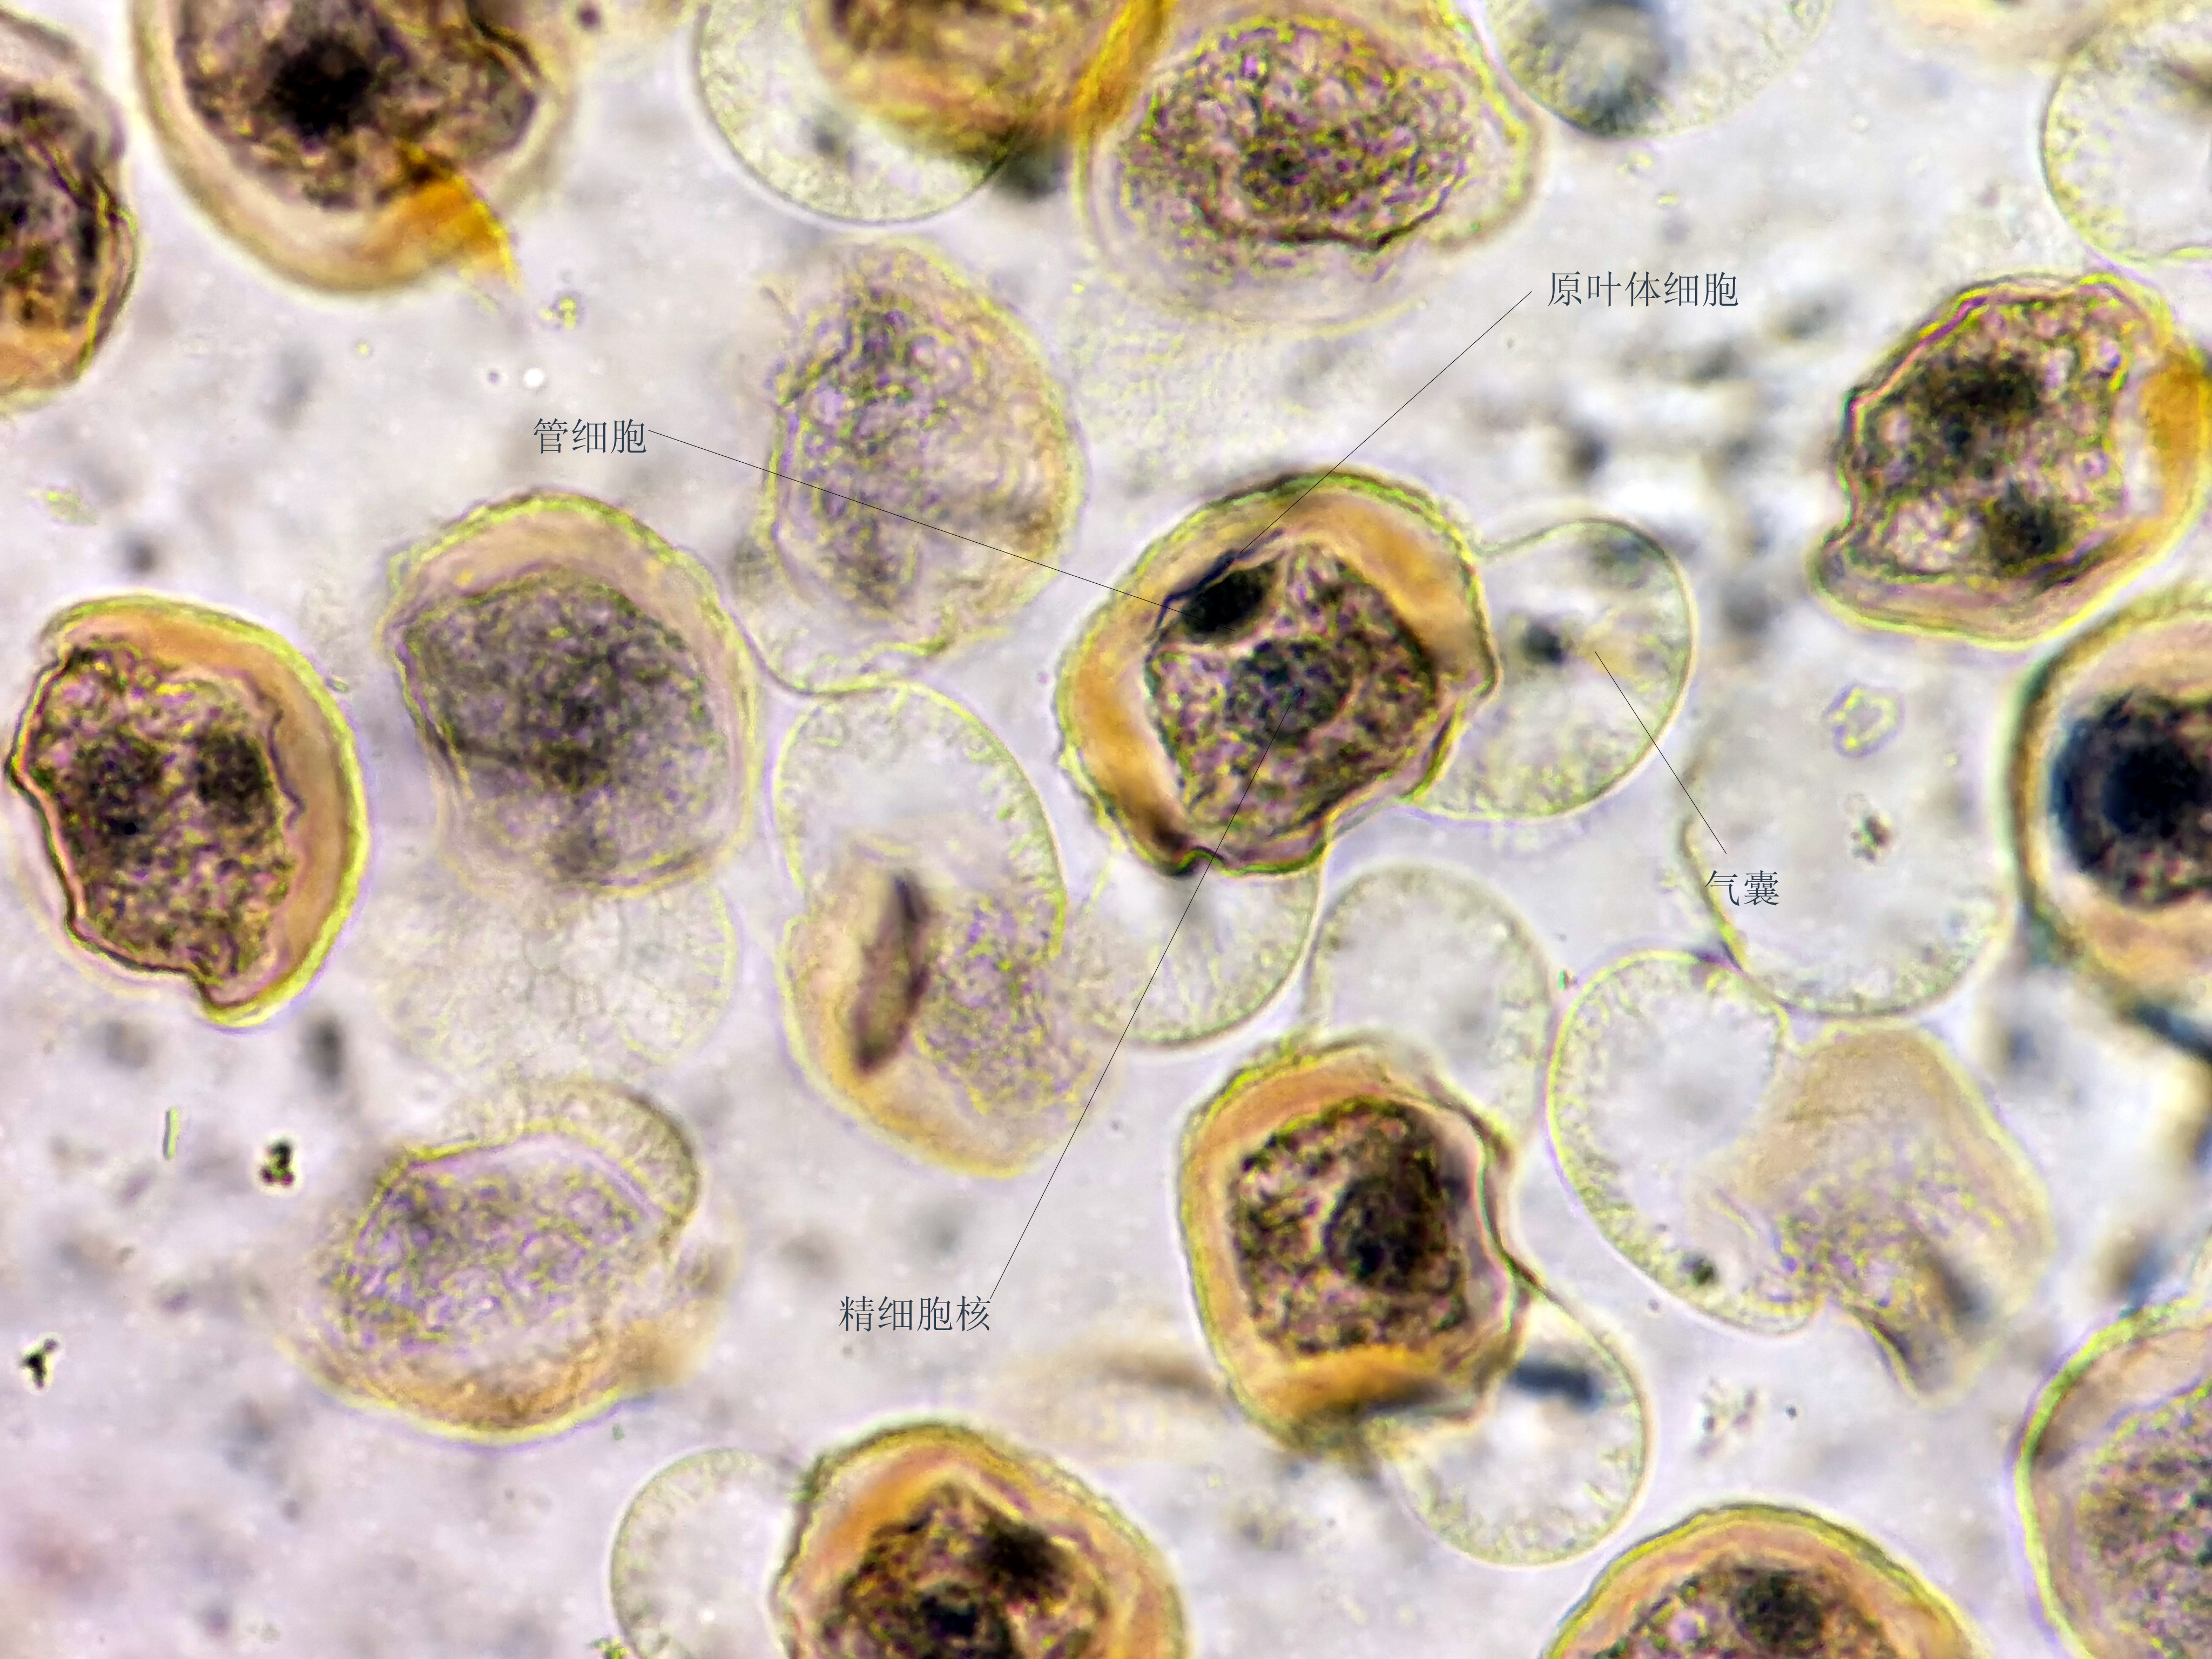
\includegraphics[scale=0.05]{src/botany/IMG_20201125_200145.jpg}\label{songxiong}}
    \subfigure[松树胚珠各部分结构]{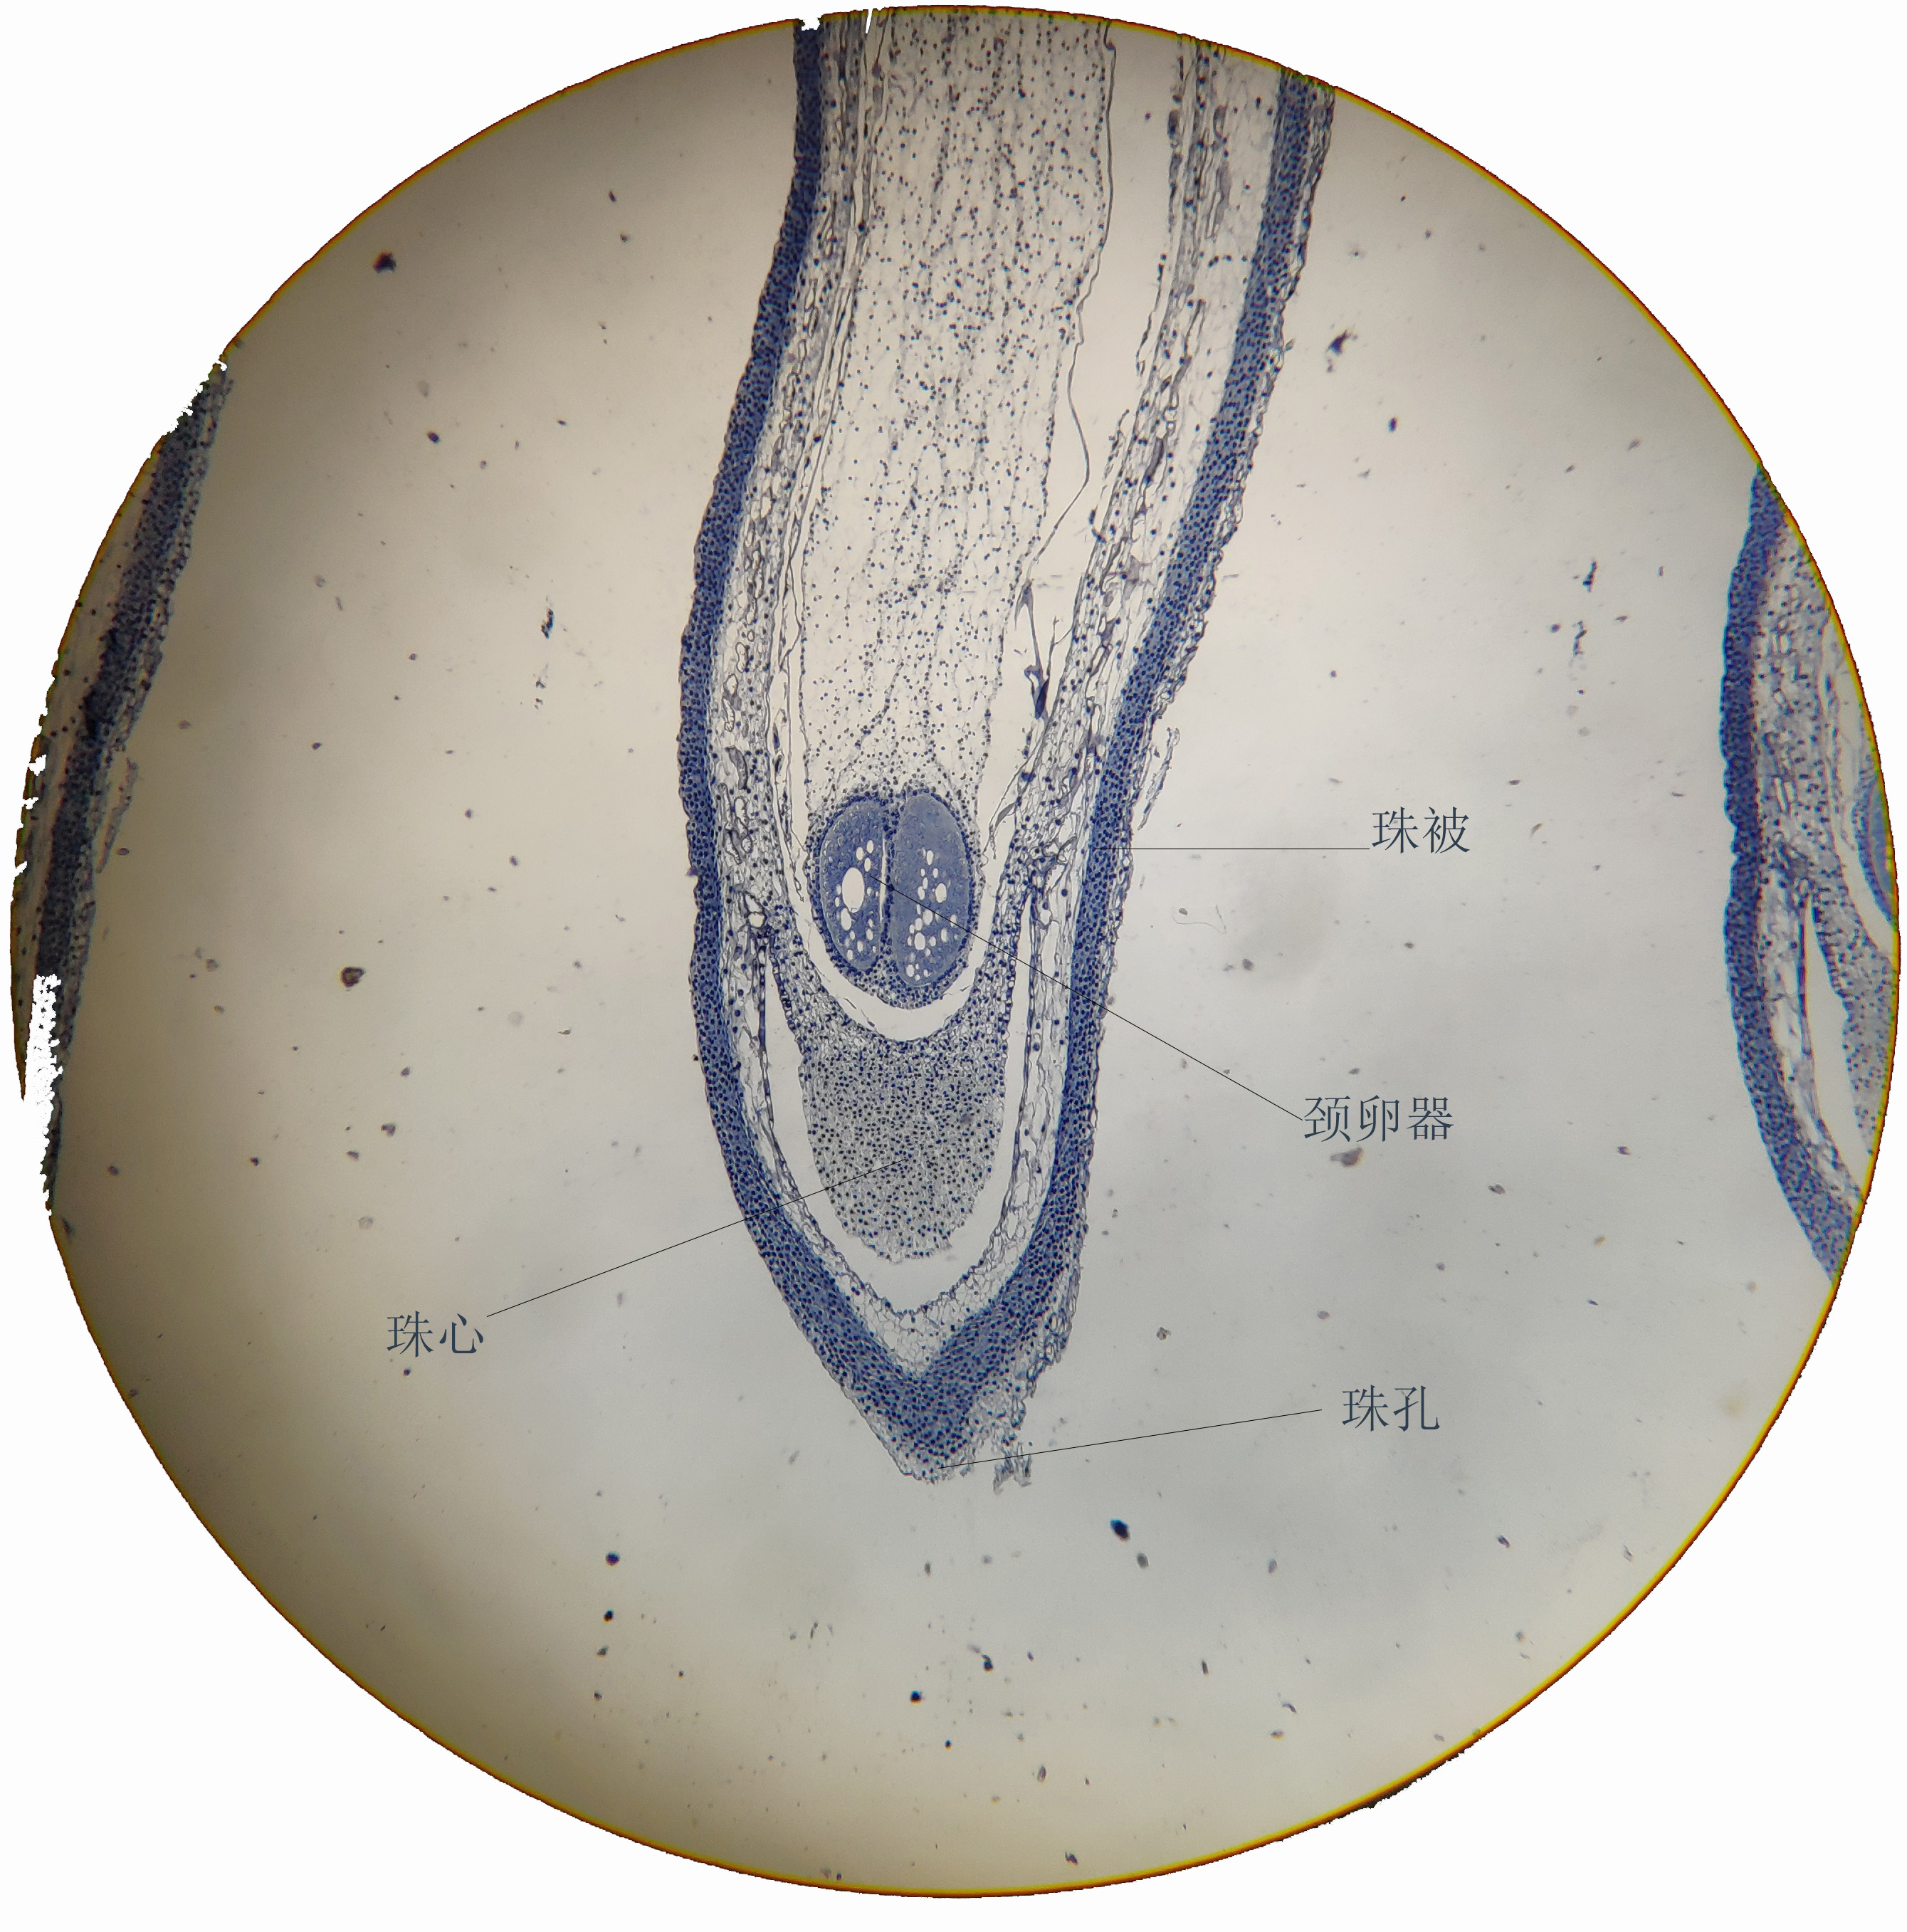
\includegraphics[scale=0.05]{src/botany/微信图片_20201218171837.jpg}\label{songpei}}
    \caption{松树生殖系统}
\end{figure} 
    \paragraph*{1.用而图或照片显示松树雄配子体结构,包括生殖细胞,粉管细胞和原叶细胞;}
    \paragraph*{答:}见\ref{songxiong}
    \paragraph*{2.用简图或照片显示松树胚珠各部分结构,包括珠被、珠心、雌配子体、颈卵器等.}
    \paragraph*{答:}见\ref{songpei}
\subsection*{讨论}
    \paragraph*{1.松树花粉与雄配子体是什么关系?}
    \paragraph*{答:}花粉即是一个成熟的配子体
    \paragraph*{2.松树种子中的胚乳是几倍体?为什么?}
    \paragraph*{答:}单倍体。因为没有双受精现象
\end{document}